\begin{figure}[htbp]
\centering
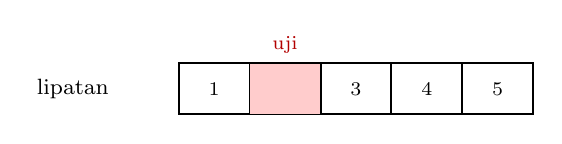
\begin{tikzpicture}[x=0.9cm,y=0.65cm]
  \foreach \f in {1,...,5} {
    \draw[thick] (\f,0) rectangle ++(1,1);
    \node[font=\scriptsize] at (\f+0.5,0.5) {\f};
  }
  \node[font=\footnotesize, anchor=east] at (0.15,0.5) {lipatan};
  \draw[fill=red!20] (2,0) rectangle ++(1,1);
  \node[font=\scriptsize, red!70!black] at (2.5,1.35) {uji};
\end{tikzpicture}
\caption{Skema validasi silang $k$-lipat ($k=5$): setiap lipatan bergantian menjadi partisi uji; skor dirata-rata untuk estimasi kinerja lebih stabil daripada satu split tunggal.}
\end{figure}
